\documentclass[12pt]{article}
\usepackage{algorithm}
\usepackage[]{algorithm2e}
\usepackage{algorithmic}
\usepackage{natbib}
\usepackage[french]{babel}
\usepackage[utf8]{inputenc}

\usepackage{amsmath}
\usepackage{graphicx}
\usepackage[colorinlistoftodos]{todonotes}
\usepackage{url}
\usepackage{hyperref}
%pour la mise en page des tableaux
\usepackage{array}
\usepackage{tabularx}
\usepackage{setspace}
\usepackage{abstract}
\usepackage[T1]{fontenc}
\usepackage[top=2cm, bottom=2cm, left=2cm, right=2cm]{geometry}
\usepackage{subfig}
\usepackage{placeins}
\usepackage{subfig}

\usepackage[utf8]{inputenc}
%régler l'espacement entre les lignes
\newcommand{\HRule}{\rule{\linewidth}{0.5mm}}

\title{rapport MAOA}
\author{luongbinhthanh}
\date{January 2019}

\usepackage{natbib}
\usepackage{graphicx}

\begin{document}

\begin{titlepage}
\begin{center}

% Upper part of the page. The '~' is needed because only works if a paragraph has started.

\includegraphics[width=0.35\textwidth]{pictures/logo.jpg}~\\[1cm]

\textsc{\LARGE Sorbonne Université (Master ANDROIDE)}\\[1.5cm]

\textsc{\Large }\\[0.5cm]

% Title
\HRule \\[0.4cm]

{\huge \bfseries Projet MAOA\\
Tournées de techniciens \\[0.4cm] }

\HRule \\[1.5cm]

% Author and supervisor
\begin{minipage}{0.4\textwidth}
\begin{flushleft} \large
\emph{Auteur:}\\
Clément \textsc{Boisson}\\
Binh Thanh \textsc{Luong}
\end{flushleft}
\end{minipage}
\begin{minipage}{0.4\textwidth}
\begin{flushright} \large
\emph{Encadrants:} \\
Pierre \textsc{Fouilhoux}\\
\end{flushright}
\end{minipage}

\vfill

% Bottom of the page
{\large \today}

\end{center}
\end{titlepage}
\tableofcontents
\newpage

\section{Introduction}
\label{S introduction}

Dans le cadre de l'UE MAOA du master Androide, nous avons effectué un projet. Ce projet est proposé par M. Fouilhoux. Il consiste en la résolution d'un problème de tournées de techniciens de manière approchée et de manière exacte. Puis nous devions ajouter des contraintes rendant le problème plus difficile à résoudre.

Une instance du problème de tournées des techniciens est un ensemble de points, parmi lesquels on trouve un entrepôt et des clients. Chaque client a une demande à satisfaire. Des véhicules vont donc partir de l'entrepôt et livrer la demande de chacun des clients puis retourner à l'entrepôt. Les véhicules ont une capacité limitée, donc il faut que la somme des demandes d'une tournée ne dépasse pas la capacité maximale des véhicules. Le but de ce problème est donc de trouver la tournée de chacun des véhicules de manière à ce que l'ensemble des tournées prennent le moins de temps possibles (il faut minimiser la somme des distances sur chaque tournée).

Ce problème réunit deux problèmes connus, le problème de sac-à-dos multiple (\textit{Bin Packing Problem}) et le problème du voyageur de commerce (\textit{Travelling Salesman Problem}). Ces deux problèmes étant NP-difficiles, le problème de tournées des techniciens est au moins autant difficile à résoudre.

Dans ce rapport, nous expliquons dans un premier temps nos méthodes de résolution pour obtenir de bonnes solutions et des solutions exactes. Puis nous expliquons ensuite comment résoudre le problème si on ajoute de nouvelles contraintes.
\section{Première partie}
\subsection{Résolution approchée}
\label{S resolution approchee}

Nous voyons dans cette partie la résolution des instances de ce problème par des heuristiques. Le but de ces heuristiques est d'obtenir de bonnes solutions proches de la solution optimale et de manière rapide. Ce cas de recherche de solutions s'applique si l'entreprise veut une solution dans l'immédiat. Pour cela, nous avons adopté une stratégie en deux parties. La première partie est de construire une solution réalisable rapidement et la deuxième est d'améliorer la solution obtenue. La première partie ne cherche donc pas une bonne solution, mais seulement une solution réalisable.

\subsubsection{Problème du sac-à-dos multiple}
\label{sub probleme du sacados}

Nous voyons ici la résolution du problème de sac-à-dos multiple (\textit{Bin Packing}) par une heuristique. Ce problème se résume à devoir résoudre le problème du sac-à-dos avec plusieurs sacs. Donc il faut remplir des sacs ayant une capacité avec des objets qui ont un poids. Le but est de minimiser le nombre de sacs utilisés. Nous avons fait le choix d'utiliser l'algorithme \textit{First Fit Decreasing} pour résoudre ce problème.

Cet algorithme prend en entrée la liste des clients triés dans l'ordre décroissant de leur demande. Il retourne une liste de listes d'entiers qui représente les indices des clients affectés à chaque véhicule. Il parcourt la liste des clients données en entrée, pour chaque client, il cherche à le placer dans la première tournée où il peut le placer. Si le client ne peut pas être placé dans une tournée, alors on crée une nouvelle tournée afin de le placer dans celle-ci. Ci-dessous le pseudo code de l'algorithme:

\begin{algorithm}[H]
    \label{A First Fit Decreasing}
    \KwData{clients: la liste des clients dans l'ordre décroissant de leur demande}
    \KwResult{l: l'affectation des clients à chaque véhicule}
    initialisation : $l = \emptyset$\\
    \For{\text{c $\in$ clients}}{
        \For{\text{t $\in$ l}}{
            \If{\text{c peut être dans t}}{
                \text{ajouter c à t}\\
                \text{continuer}
            }
        }
        \If{\text{c n'a pas été ajouté}}{
            \text{créer une liste vide t'}\\
            \text{ajouter c à t'}\\
            \text{ajouter t' à l}
        }
    }
    \caption{First Fit Decreasing}
\end{algorithm}

Cet algorithme renvoie la répartition des clients pour chaque véhicule. Il est 2-approché et a une complexité de $O(n \log(n))$ où n est la taille de l'entrée. A la fin de l'exécution de cet algorithme, nous avons la liste des clients de chaque tournée. Nous devons maintenant optimiser l'ordre des clients dans chaque tournée (voir la partie \ref{sub voyageur de commerce}).

\subsubsection{Problème du voyageur de commerce}
\label{sub voyageur de commerce}

Dans cette sous-partie, nous étudions la résolution du problème du voyageur de commerce (\textit{Travelling Salesman Problem}) par une heuristique. Pour notre problème, il faut résoudre le problème du voyageur de commerce pour chacune des tournées, à savoir trouver un cycle passant par tous les clients de façon à minimiser la somme des distances parcourues. Pour résoudre ce problème, nous avons implémenté l'algorithme \textit{Nearest Insertion}.

Cet algorithme prend en entrée la liste des clients pour chaque tournée (voir partie \ref{sub probleme du sacados}). Il retourne une liste de listes d'entiers qui représente les indices des clients affectés à chaque tournée dans l'ordre dans lequel la tournée doit être effectuée. Voici le pseudo code de l'algorithme:

\begin{algorithm}[H]
    \label{A Nearest Insertion}
    \KwData{l: l'affectation des clients à chaque véhicule}
    \KwResult{l2: la liste des tournées}
    \For{\text{t $\in$ tournées}}{
        Choisir un client i le plus proche du dépôt, former la tournée 0-i-0\\
        Clients de t $\gets$ Client de t \textbackslash \{i\} \\
        \While{\text{Clients de t} $\neq \emptyset$}{
        k \in \text{Clients de t} : d(k,t) = $min_{i \in t}$ d(i,t) \\
        \text{Trouver (i,j)} : $\delta$ f = $c_{ik}$ + $c_{kj}$ - $c_{ij}$ \text{soit minimal}\\
        \text{Insérer k entre i et j}\\
        \text{Clients de t} \gets \text{Clients de t} \textbackslash \{k\}\\
        }
    }
    \caption{Nearest Insertion}
\end{algorithm}

Cet algorithme renvoie la liste des tournées. Il est 2-approché pour chaque véhicule et a une complexité de $O(n^2)$ où n est le nombre de clients par tournée. La solution retournée est loin de la solution optimale. Comme évoqué dans l'introduction de la partie \ref{S resolution approchee}, nous cherchons une solution réalisable rapidement afin de partir de celle-ci pour en trouver une meilleure. Dans ce but, nous utilisons un algorithme de recuit simulé (voir partie \ref{sub recuit simule}).

\subsubsection{Recherche locale}
\label{sub recherche locale}
Pour améliorer les tournées, nous appliquons ensuite une recherche locale avec une liste de tabou. Le but de la recherche locale est de réduire le coût de chaque tournée en y permutant deux clients. Nous gardons en mémoire une liste de tabou pour éviter d'être bloqué dans un optimum local.


\subsubsection{Amélioration par recuit simulé}
\label{sub recuit simule}
A la fin des algorithmes évoqués dans les parties \ref{sub probleme du sacados} et \ref{sub voyageur de commerce}, nous obtenons une solution réalisable. Cette solution étant très loin de la solution optimale, il nous faut l'améliorer. Pour cela, nous avons implémenté un algorithme de recuit simulé.

Cet algorithme prend en entrée une solution réalisable et retourne une solution réalisable et proche de la solution optimale. Voici les arguments de cet algorithme:

\begin{itemize}
    \item $k_{max}$ : Le nombre d'itérations maximal que l'algorithme va faire, elle vaut $2000$ dans notre méthode
    \item T : la température initiale de l'algorithme, elle vaut $1000$ dans notre méthode
    \item $\alpha$ : le coefficient de mise-à-jour de la température, à chaque itération: $T \gets T \times \alpha$
    \item $energy_{min}$ : l'énergie minimale de la solution trouvée, si l'algorithme trouve une solution en dessous de $energy_{min}$, alors il s'arrête
\end{itemize}\\

L'algorithme de recuit simulé prend la solution courante, et si le nombre $k$ d'itérations est inférieur à $k_{max}$, alors il va chercher le voisin de la solution courante. Pour trouver le voisin, on change un client de tournée, on fait une permutation de deux clients dans une même tournée, on ajoute une tournée ou on supprime une tournée vide. Ces façons de trouver un voisin sont tirés aléatoirement avec respectivement $1/3$, $1/3$, $1/6$ et $1/6$ de chance d'être pris. Ensuite l'algorithme compare les énergies des solutions. L'énergie est calculée de la manière suivante:

\begin{equation}
\label{equation energie}
    \sum_{t \in tournees} distance_t + 100 \times \max \{0, (\#tournee - m)\}
\end{equation}

Si l'énergie du voisin est meilleure (plus basse), alors on remplace la solution courante par le voisin. Sinon on remplace la solution courante par le voisin avec une probabilité de $\exp(\delta energy / T)$ où $\delta energy$ est la différence entre l'énergie du voisin et l'énergie de la solution courante. De plus, on garde en mémoire la meilleure solution rencontrée, c'est cette solution qui sera retournée. Voici le pseudo code de l'algorithme:

\begin{algorithm}[H]
    \label{A Simulated Annealing}
    \KwData{s: la solution à améliorer}
    \KwResult{s': la meilleure solution rencontrée}
    \text{initialisation : k = 0 et $energy_{s}$ = energy(s)}\\
    \While{\text{k < $k_{max}$ ou $energy_s$ < $energy_{min}$}}{
        \text{sn $\gets$ voisin(s) et $energy_{sn}$ = energy(sn)}\\
        \text{p est tiré aléatoirement entre 0 et 1}\\
        \If{\text{$energy_{sn}$ < $energy_{s}$ ou p < $\exp(\delta energy / T)$}}{
            \text{s $\gets$ sn}\\
            \text{$energy_{s}$ $\gets$ $energy_{sn}$}
        }
        \If{\text{$energy_{sn}$ < $energy_{s'}$}}{
            \text{s' $\gets$ sn}\\
            \text{$energy_{s'}$ $\gets$ $energy_{sn}$}
        }
        \text{k $\gets$ k + 1}\\
        \text{T $\gets$ T $\times$ $\alpha$ }
    }
    \caption{Simulated Annealing}
\end{algorithm}

A la suite de l'exécution de cet algorithme, nous obtenons une solution proche de la solution optimale. Nous avons donc une bonne solution obtenue rapidement à la suite des trois algorithmes décrit dans les parties \ref{sub probleme du sacados}, \ref{sub voyageur de commerce} et \ref{sub recuit simule}. Par exemple, nous obtenons, pour l'instance \texttt{A-n32-k5}, une solution autour de 1800 à la suite des algorithmes des parties \ref{sub probleme du sacados} et \ref{sub voyageur de commerce}, alors que l'on trouve une solution proche de 900 après l'algorithme de recuit simulé. La solution optimale de l'instance \texttt{A-n32-k5} est à 787 (voir la partie \ref{result}).
\subsection{Résolution exacte par \texttt{PLNE}}
\label{S resolution exacte par plne}
Le système d'équations ci-dessous nous permet de modéliser le \texttt{VRP} sans la capacité :
\[\text{Min} \sum_{(i, j) \in A} c_{ij}x_{ij}\]

\[\begin{cases}
{\mathlarger\sum_{j=1}^{n}} x_{0j} \leq m \\
{\mathlarger\sum_{i=1}^{n}} x_{i0} \leq m\\
{\mathlarger\sum_{j=0}^{n}} x_{ij} \leq m, \forall i \in \mathcal{N}_{\mathcal{C}}\\
{\mathlarger\sum_{i=0}^{n}} x_{ij} \leq m, \forall j \in \mathcal{N}_{\mathcal{C}}\\
x_{ij} \in \{0,1\}, \forall (i, j) \in A
\end{cases}\]

Nous utilisons ensuite \texttt{Cplex} pour résoudre ce système. La solution obtenue est une répartition des clients dans des tournées qui minimise la fonction objectif. Cependant ces tournées ne contiennent pas forcément le dépôt ou dépassent la capacité. Afin de briser ces tournées non réalisables, nous ajoutons, au fur et à mesure, les contraintes suivantes qui nous permettent de supprimer ces tournées non réalisables.
\[
\sum_{i \in W} \sum_{j \in \{0, 1, ..., n\} \textbackslash W } x_{ij} \geq {\Bigg\lceil} \dfrac{\sum_{i \in W} d_i}{Q} {\Bigg\rceil} \forall W \subset \{1, ..., n\}, W \neq \emptyset
\]

A chaque fois que le solveur détecte une solution valide, nous analysons chacune des tournées de cette solution. Si une tournée ne passe pas par le dépôt, cette contrainte est ajoutée et force la tournée à avoir au moins un arc sortant ce qui a pour conséquence de briser le cycle. De plus, si une tournée passe par le dépôt, nous vérifions que la somme des demandes des clients ne dépasse pas la capacité. Si cette somme dépasse la capacité du véhicule cette tournée n'est pas réalisable. Cette contrainte est alors ajoutée et indique le nombre minimum de véhicules pour servir tous les clients de cette tournée.
\subsection{Résultats expérimentaux}
\label{result}
Nous analysons ici les premiers résultats de nos deux méthodes de résolution. Pour la résolution approchée, nous affichons ci-dessous les solutions trouvées à différentes étapes pour l'instance \texttt{A-n32-k5}:

\begin{center}
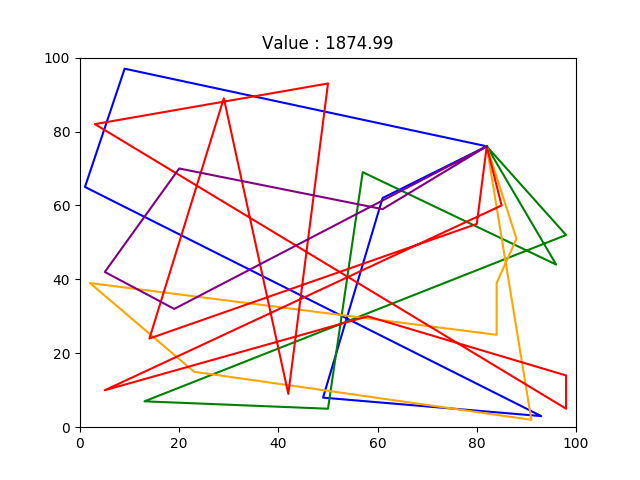
\includegraphics[width=0.32\linewidth]{pictures/image5.png}
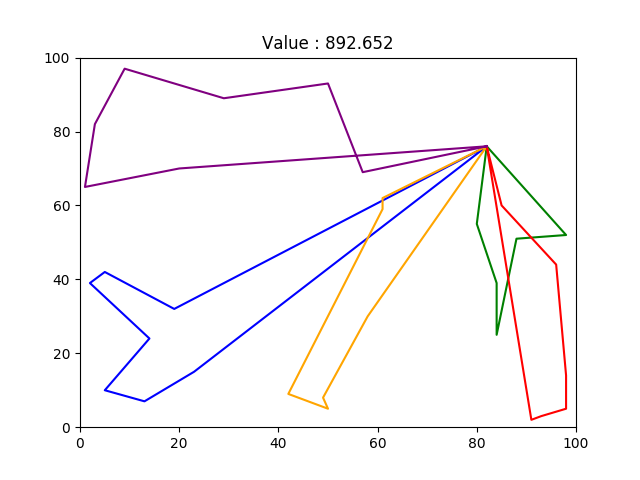
\includegraphics[width=0.32\linewidth]{pictures/image2.png}
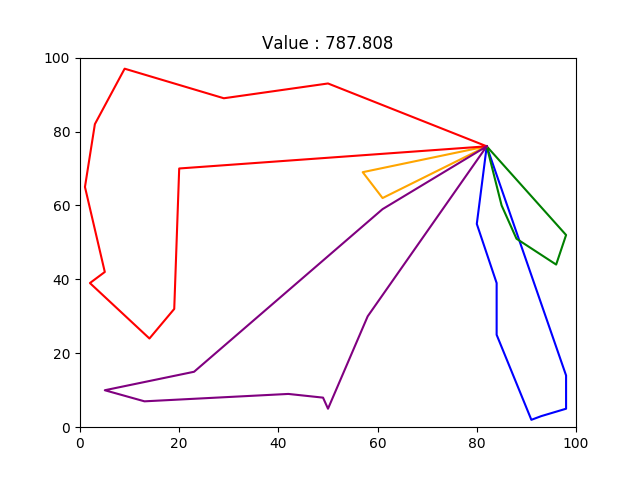
\includegraphics[width=0.32\linewidth]{pictures/image3.png}
\captionof{figure}{Tournées obtenues par : a) Construction b) Recuit simulé c) PLNE}
\end{center}

Dans la figure ci-dessus, nous pouvons voir en a) la solution obtenue après l'étape de construction. Cette solution est très éloignée et a une valeur de 1874. En b), nous avons la solution obtenue après l'algorithme du recuit simulé. Cette solution est bien plus approchée avec une valeur de 892. En c), nous avons la solution optimale avec une valeur de 787. De ces figures, nous pouvons voir que le recuit simulé améliore notre solution de départ et retourne une solution assez proche de la solution optimale. On peut notamment reconnaître des suites de clients dans certaines tournées.\\

Dans la figure ci-dessous, nous comparons les résultats obtenus par l'heuristique de construction, le recuit simulé et la résolution exacte \href{http://vrp.atd-lab.inf.puc-rio.br/index.php/en/}{des instances de type P}. Nous limitons le solveur à 300 secondes pour chaque instance.

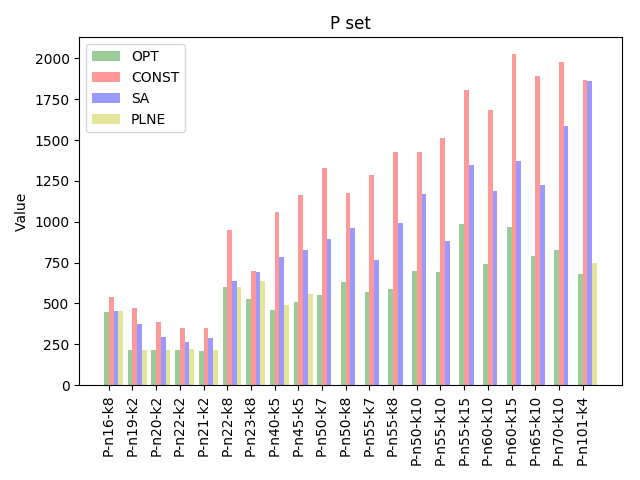
\includegraphics[width=0.8\textwidth]{pictures/image1.png}

Du fait de limiter le solveur à 300 secondes, nous remarquons que nous n'obtenons pas de résultat sur les grandes instances. Cela s'explique du fait que le nombre de contraintes de coupes augmente exponentiellement avec la taille de l'instance. Nous constatons que le recuit simulé renvoie des résultats beaucoup plus proche de l'optimum que l'heuristique de construction. Dans les cas plus difficiles, l'heuristique de recuit simulé nous donne des solutions réalisables avec un temps rapide. Pour les grandes instances, la résolution exacte prend plus de temps, mais donne de meilleurs résultats.
\section{Deuxième partie}
Dans cette partie, nous souhaitons rendre le problème plus proche de la réalité. C'est la raison pour laquelle nous ajoutons des contraintes supplémentaires.

\subsection{Ajout du temps de travail}
\label{S ajout du temps de travail}
Dans un premier temps, nous avons ajouté des contraintes sur le temps de travail. De ce fait, nous limitons le temps de travail de chaque technicien et nous pénalisons le temps de travail supplémentaire dans la fonction objectif.

De ce fait, nous définissons un temps de travail maximal $d_{max} = \dfrac{1.5\sum_{j=1}^{n} c_{0j}}{m}$ pour chaque technicien. Pour chaque tournée, nous ajoutons dans la fonction objectif un terme qui est égale à $max(c_{tournée} - d_{max}, 0)$.

Nous remarquons que l'ajout de cet aspect est équivalent au problème initial, sauf que la fonction objectif est modifiée. La résolution du problème avec cette nouvelle contrainte n'est donc pas intéressante. Donc, nous ne l'avons pas étudiée en profondeur.
\subsection{Ajout de compétences}
\label{S ajout de competences}
Afin d'essayer d'augmenter la complexité du problème et de le rapprocher du réel, nous introduisons ici la compétence des techniciens. Nous disposons de 2 compétences A \& B et nous attribuons les compétences aux techniciens de manière suivante :
\begin{itemize}
    \item $\lfloor$20\%$\rfloor$ des techniciens sont des 2 compétences A et B
    \item $\lfloor$40\%$\rfloor$ de compétence A
    \item $\lfloor$40\%$\rfloor$ de compétence B
    \item le reste n'a pas de compétence spécifique
\end{itemize}
\\

Les clients ont aussi des demandes spécifiques aux différents services. Voici la répartition des clients:
\begin{itemize}
    \item 15\% des deux services A \& B
    \item 30\% du service A
    \item 30\% du service B
    \item 15\% pas de service
\end{itemize}
\\

Des relations existent entre les différentes compétences. En effet, un client ayant besoin les deux services ne peut être satisfait que par un techniciens ayant les deux services. De plus, un client ayant besoin du service A (respectivement B) doit être servi par un technicien ayant le service A (respectivement B) ou les deux services A \& B. Les clients n'ayant pas besoin de compétence peuvent être servi par n'importe quel technicien.

Nous pénalisons dans la fonction objectif le fait qu'un client soit servi par un mauvais technicien par un terme qui est 3 fois la distance entre le dépôt et ce client. Par exemple, un client A servi par un technicien B ou un client A \& B servi par un technicien B.\\


Nous avons modifié la structure de données pour qu'elle prenne en compte ces compétences. Pour cela, comme dans la partie \ref{sub probleme du sacados}, nous trions les clients en ordre décroissant de la demande. En suite, nous mettons les clients de type A \& B dans les tournées A \& B, si le nombre de tournées de ce type n'est pas suffisant, nous mettons le reste des clients A \& B de côté. La même procédure est appliquée pour les clients de type A (respectivement B) avec les tournées A (respectivement B). Enfin, tous les clients restant sont placés dans les tournées sans prendre en compte les compétences avec l'algorithme \textit{First Fit Decreasing}.

Les étapes suivantes de l'heuristique sont inchangées car elles évaluent les tournées avec la fonction objectif qui est déjà implémentée et qui prend en compte les pénalités des clients mal servi.
 \newpage
\begin{center}
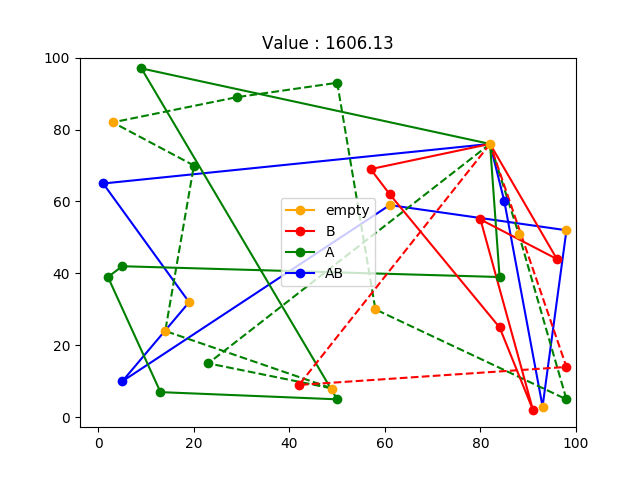
\includegraphics[width=0.49\linewidth]{pictures/image4.png}
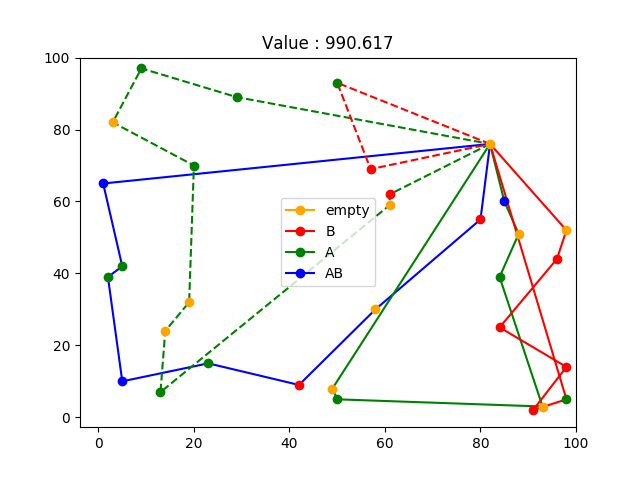
\includegraphics[width=0.49\linewidth]{pictures/image6.png}
\captionof{figure}{Tournées obtenues par heuristiques : a) Construction b) Recuit simulé pour \texttt{A-n32-k5}}
\end{center}

Nous observons dans la figure ci-dessus les solutions retournées à différentes étapes de l'heuristique. En a), nous pouvons voir la solution retournée par l'heuristique de construction, elle a une valeur de 1606. En b), nous avons la solution retournée par le recuit simulé avec une valeur de 990. Ce que nous pouvons remarquer dans cette figure c'est que la valeur de la solution est meilleur après l'application du recuit simulé. Nous constatons que les clients sont globalement attribués dans les service correspondant.
\\

Ensuite, nous avons modifié la PLNE pour qu'elle soit adaptée à ce problème. En ajoutant une troisième dimension k aux variables $x_{ij}$. Nous fixons le nombre de tournées à m. Une autre variable, $p^k_{0j}$, est ajoutée dans la fonction objectif, elle est décrite de la manière suivante :
\[
p^k_{0j} =
\begin{cases}
\text{distance entre le dépôt et le client j s'il est servi dans la mauvaise tournée k}\\
0 \text{ sinon}
\end{cases}
\]
\newpage

La PLNE devient :
\[\text{Min} \sum_{(i, j) \in A} (c^k_{ij} + 3p^k_{0j})x^k_{ij}\]

\[\begin{cases}
{\mathlarger\sum_{j=1}^{n}} x^k_{0j} = 1, \forall k \in \{0, ..., m\} \\
{\mathlarger\sum_{i=1}^{n}} x^k_{i0} = 1, \forall k \in \{0, ..., m\} \\
{\mathlarger\sum_{k=0}^{m}} x^k_{0j} \leq 1, \forall j \in \{0, ..., n\}\\
{\mathlarger\sum_{k=0}^{m}} x^k_{i0} \leq 1, \forall i \in \{0, ..., n\}\\
{\mathlarger\sum_{j=0}^{n}} x^k_{ij} \leq 1, \forall i \in \{0, ..., n\}, \forall k \in \{0, ..., m\}\\
{\mathlarger\sum_{i=0}^{n}} x^k_{ij} \leq 1, \forall j \in \{0, ..., n\}, \forall k \in \{0, ..., m\}\\
{\mathlarger\sum_{k=0}^{m}}{\mathlarger\sum_{j=0}^{n}} x^k_{ij} = 1, \forall i \in \{0, ..., n\}\\
{\mathlarger\sum_{k=0}^{m}}{\mathlarger\sum_{i=0}^{n}} x^k_{ij} = 1, \forall j \in \{0, ..., n\}\\
x^k_{ij} \in \{0,1\}, \forall (i, j) \in A, \forall k \in \{0, ..., m\}
\end{cases}\]

Ces contraintes modélisent l'ensemble du problème mais elles ne sont pas suffisantes pour avoir plus d'information sur chaque tournée. Les valeurs retournées dans la fonction \textit{callback} ne nous permettent pas de couper les points.

Avec cet aspect, le problème devient plus facile pour les heuristiques. En effet, le problème est moins "combinatoire" parce que le seul moyen de résoudre ce problème est de placer au mieux les clients dans les tournées correspondantes à leur besoin.
\section{Conclusion}
\label{S conclusion}

Ce projet nous a permis de mettre en pratique les connaissances acquises en cours, comme les algorithmes de coupes. Le projet est réaliste et peut très bien s'appliquer dans la réalité.

De plus, il met en évidence les différences entre les résolutions approchées et les résolutions exactes. En effet, la résolution approchée est rapide mais ne renvoie pas la solution optimale. En revanche, la résolution exacte est plus longue, mais retourne la solution exacte. Nous pensons donc que les deux méthodes doivent être utilisées selon les conditions. Si nous disposons d'assez de temps, la résolution exacte reste la meilleure option. Au contraire, si le temps nous manque, la résolution approchée est plus adaptée.



\end{document}
